% siminos/gudorf/thesis/chapter/KSe.tex
% $Author: predrag $ $Date: 2020-05-25 15:18:45 -0400 (Mon, 25 May 2020) $

% called by
%           siminos/spatiotemp/chapter/spatiotemp.tex
%           siminos/tiles/GuBuCv17.tex

%\section{\KSe}
%\label{sect:KSe}
% Predrag                                           2019-03-19

The \KS\
equation\rf{KurTsu76,siv}, which arises in the
description of stability of flame fronts, reaction-diffusion systems and
many other physical settings\rf{KNSks90,ReChMi07}, is one of the simplest
nonlinear PDEs that exhibits {\spt}ly chaotic behavior. In one
space dimension it is defined on the doubly infinite spacetime plane
\index{Kuramoto-Sivashinsky!system}
\beq
    u_\zeit  + u\,u_\conf + u_{\conf \conf} + u_{\conf \conf \conf \conf} = 0
    \,,\quad
    (\conf,\zeit) \in \reals^2
    \,,
\ee{e-ks}
where  $t$ is the time, $\conf$ is the spatial coordinate, subscripts
$(\cdot)_\conf$ and $(\cdot)_t$ denote partial derivatives with respect
to $\conf$ and $t$, and the field $u=u(\conf,\zeit)$ can be thought of as
the `flame front velocity' at the spacetime point $(\conf,\zeit)$.
Occasionally the form of \refeq{e-ks} will include a coefficient $\nu$ on
the ``hyper-viscosity'' term, \ie, $\nu u_{\conf \conf \conf \conf}$. We have
exchanged this control parameter for non-dimensional length via the relation
\beq
\speriod{} = \frac{L}{2\pi \sqrt{\nu}}\,,
\eeq
and setting $\nu=1$. This seems to be the more natural choice as solutions have on
the order of $\speriod{}$ number of wavelengths at any given time; this
allows for quick interpretation and verification of figures of scalar
fields later on. We do note that this may be a frustrating choice as
there is much literature in which $L=22$ is the spatial domain size
being reported on\rf{BudCvi15,DCTSCD14,DingCvit14,SCD07,GOSW19}.
This translates to $\speriod{22}\approx 3.50$ for reference. An alternative
choice would be to set the scale in terms of the most unstable wavelength
$\tilde{L}^* = \frac{L}{2\pi\sqrt{2}}$



%%%%%%%%%%%%%%%%%%%%%%%%%%%%%%%%%%%%%%%%%%%%%%%%%%%%%%%%%%%%%%
\begin{figure} %[t]
\begin{center}
%{figs/ks_largeL_cbar_200.eps} % RLD: longer orbit (to make appearance similar to ks_L22_long_orbit.eps)
%{figs/ks_largeL_cbar.eps}
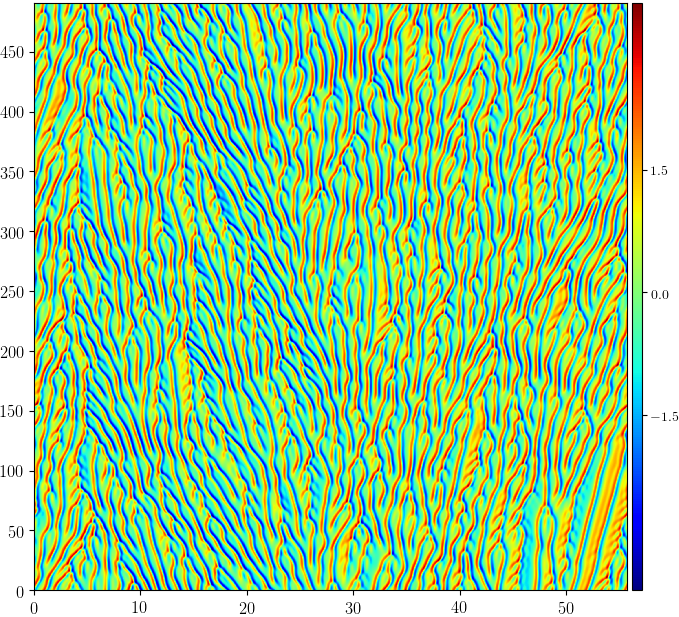
\includegraphics[width=0.9\textwidth]{MNG_u_largeL}
\end{center}
\caption{
A typical {\spt} ``steady state turbulence'' \KS\ solution $u(\conf,\zeit)$,
integrated forward in time on a periodic domain of size
$\speriod{}\approx 79.57$
(after the initial transient has died out).
The most unstable wavelength $2\pi\sqrt{2}$ of the u=0 \eqv\ (see
\refsect{sect:KSu0equiT}) is an estimate the mean spatial wavelength of
the turbulent \KS\ flow, so there are approximately 55 wiggles across the
spatial domain at any instant in time.
The color bar indicates the color scheme for $u(\conf,\zeit)$, used also
for the subsequent figures of this type.
     } \label{f:ks_largeL}
\end{figure}
%%%%%%%%%%%%%%%%%%%%%%%%%%%%%%%%%%%%%%%%%%%%%%%%%%%%%%%%%%%%%%%%%%

There is  much interest in \KSe\ because \refeq{e-ks}
is a 1\dmn\ PDE analogue of the 3\dmn\ \NS\ PDEs
\beq
\dfrac{\partial \bv}{\partial t} + (\bv \cdot \nabla) \bv
\,{\color{red}-}\,\frac{1}{R} \nabla ^2 \bv + (\cdots)	
% -\nabla p + \mathbf{f}    \,,\qquad \nabla \cdot \bv = 0,
\,=\, 0
\,,\qquad
(\bx,\zeit) \in \reals^4
\,,
\ee{NSe}
where  $(\cdots)$ stands for various forcing terms. Holmes, Lumley and
Berkooz\rf{Holmes96} offer a delightful discussion of why \KS\ system
deserves study as a staging ground for studying turbulence in
full-fledged Navier-Stokes boundary shear flows. First, high quality
simulations of \NS\rf{channelflow,WillisPipe17} are much harder than \KS\
simulations\rf{ks05com}. Second, and the real reason why in this paper we
introduce the reader to the {\spt} theory of turbulence using \KS\ as an
example, is that it is very hard to visualize 3\dmn\ velocity field at
every 3\dmn\ spatial pointand at every instant in time. In contrast,
\spt\ visualization of \KS\ as color-coded magnitude of 1\dmn\ velocity
field $u$ over the spacetime $(\conf,\zeit)$, as in \reffig{f:ks_largeL},
is immediate.

It suffices to inspect a single generic \spt\ solution of \KSe\, such as
\reffig{f:ks_largeL}, to be almost always able to recognize any other solution $u$ as
a solution of \KSe.
Indeed, the goal of this paper is to explain \emph{why}, by deriving the
alphabet of admissible patterns from the \KSe, and assigning a unique
{\spt} ``word'' to any solution that can be seen embedded into
the chaotic (turbulent) attractor (inertial manifold).
It is intuitive by inspection that there is a typical spatial ``mean
wavelength'' (\refsect{sect:KSu0equiT}) and a typical time scale, that
the patterns are exponentially decorrelated beyond several space and time
scale units (\refsect{exam:KurSivTempstab} and \refsect{sect:KSu0equiS}),
and that all statistical averages, such as energies
and dissipation rates, should be extensive (see \refsect{sect:KSenerg}).
